\documentclass[8pt,a4paper]{beamer}
\usepackage[utf8]{inputenc}
\usetheme{Warsaw}
\setbeamercovered{transparent}
\useoutertheme[subsection=false]{smoothbars}


\usepackage{amssymb}
\usepackage{graphicx}
\usepackage{fancyhdr}
\usepackage{amsmath}
\usepackage{answers}
\usepackage{lastpage}
\usepackage{enumerate}
\usepackage{array}
\usepackage{tikz}
\usepackage{tikz-3dplot}
\usepackage{array,multirow,makecell}
\usepackage{mdwlist}
\usepackage{systeme}
\usepackage{relsize} 
\usepackage{siunitx}
\usepackage{multirow}
\usepackage{lscape}
\usepackage{makecell}
\usepackage{xcolor}
\usepackage{setspace}
\usepackage{lipsum} 
\usepackage{hyperref} 
\usepackage[french]{babel} 
\usepackage{multicol}
\usepackage{url}
\usepackage{eurosym}
\usepackage{hyperref}
\usepackage{breakurl}
\numberwithin{figure}{section}
\usepackage{caption}
\usepackage{graphicx}

\setbeamertemplate{headline}{}

\renewcommand{\listfigurename}{}

\definecolor{onered}{RGB}{8,70,114}
\usecolortheme[named=onered]{structure}

\title[\thepage/\pageref{LastPage}]{Restauration d'Images Sous-marines}
\author[CSC\_4IM01\_TP ] {\small Fouad KHELIFI\\ Hortense BONNEAU}
\institute[Télécom Paris]{\large Télécom Paris}
\date[4IM01] {CSC\_4IM01\_TP : Introduction au Traitement des Images}
\titlegraphic { 
\begin{tikzpicture}[overlay,remember picture]
\node[above=8mm] at (current page.-90){
    
\includegraphics[width=3cm]{TP.png}

};
\end{tikzpicture}
}

\begin{document}

\begin{frame}[plain]
\Large \titlepage
\end{frame}

\begin{frame}{Table des Matières}
  \tableofcontents 
\end{frame}

\section{État de l'Art du Traitement des Images Sous-Marines}
\subsection{Introduction}
\frame{\tableofcontents[currentsection]}
\begin{frame}{Introduction}
\begin{columns}
\begin{column}{7cm}
\par Le traitement des images sous-marines est crucial pour surmonter les limitations inhérentes à l'environnement aquatique, comme la faible visibilité, le flou, et la dominante bleue causée par l'absorption et la diffusion de la lumière. Ces défis limitent la portée visuelle et la qualité des images, en particulier à de grandes profondeurs ou dans des eaux troubles. Les méthodes proposées pour résoudre ces problèmes se répartissent en deux catégories principales : \textbf{la restauration d'image} et \textbf{l'amélioration d'image}, chacune ayant des applications et des contraintes spécifiques.
\end{column}
\begin{column}{3cm}
\begin{center}
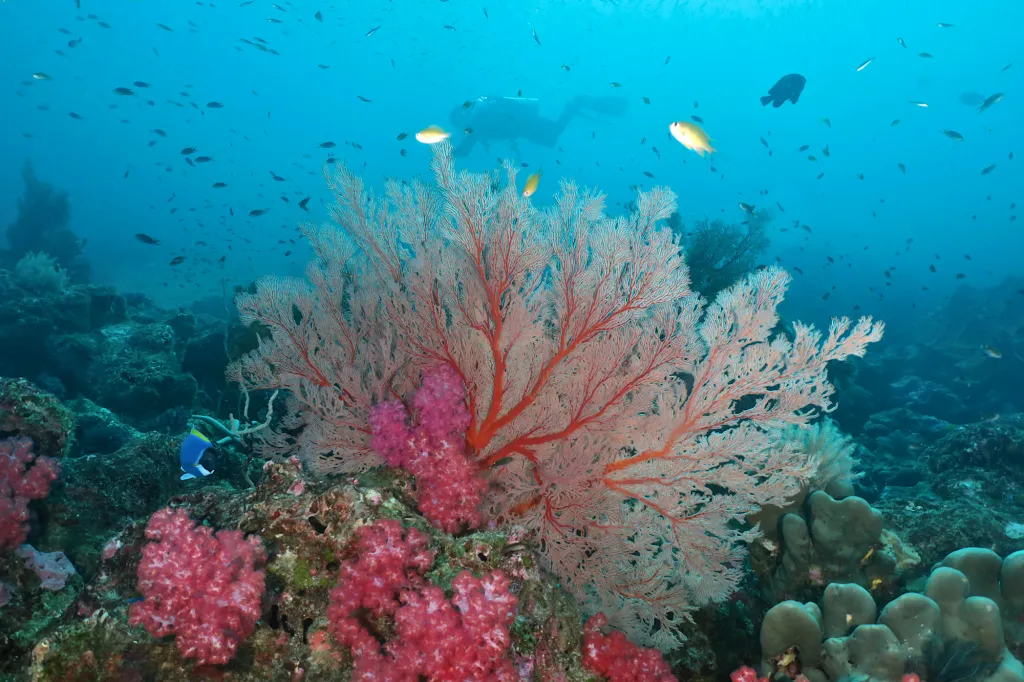
\includegraphics[width=3cm]{image010.png}
\end{center}
\end{column}
\end{columns}
\end{frame}

\subsection{Méthodes de Restauration d'Image}
\begin{frame}{Méthodes de Restauration d'Image}
\par Les images sous-marines subissent une dégradation importante causée par l'absorption et la diffusion de la lumière. L'absorption réduit progressivement l'énergie lumineuse, supprimant les couleurs selon leur longueur d'onde (par exemple, le rouge disparaît après environ 3 mètres). La diffusion, quant à elle, provoque un flou et diminue le contraste, amplifiant le \textit{voile} visuel. Les techniques de restauration compensent ces effets par :
\vspace{3mm}
\begin{itemize}
\item[$\bullet$] \textbf{Modélisation physique :} Exploite les propriétés optiques de l'eau (absorption, diffusion) et des fonctions de transfert pour corriger flous et pertes de contraste.
\item[$\bullet$] \textbf{Déconvolution :} Applique des filtres, comme celui de Wiener, basés sur des fonctions mesurant la propagation lumineuse pour restaurer les détails.
\item[$\bullet$] \textbf{Analyse de polarisation :} Isolant la lumière diffusée grâce à des filtres polarisants, elle réduit les voiles optiques et améliore le contraste.
\end{itemize}
\vspace{3mm}
Ces méthodes, bien que précises, dépendent fortement des caractéristiques de l’environnement aquatique.
\end{frame}

\subsection{Méthodes d'Amélioration d'Image}
\begin{frame}{Méthodes d'Amélioration d'Image}
\par Les techniques d’amélioration visent à optimiser la qualité visuelle des images sans nécessiter de modèles physiques complexes. Elles se concentrent sur la correction des couleurs, l'ajustement des contrastes et la suppression des dominantes chromatiques.
\vspace{3mm}
\begin{itemize}
\item[$\bullet$] \textbf{Espace $l\alpha\beta$ :} En convertissant les images dans un espace de couleur perceptuel, cette approche ajuste indépendamment la luminosité, la teinte et la saturation pour atténuer la dominante bleue et rehausser les détails visuels.
\item[$\bullet$] \textbf{Automatic Color Equalization (ACE) :} Inspirée de la perception humaine, cette méthode ajuste automatiquement les couleurs et le contraste pour compenser les dominantes dues à l’absorption sous-marine, offrant des images plus équilibrées et naturelles.
\end{itemize}
\vspace{3mm}
On met en avant et implémente spécifiquement ces deux méthodes, en raison de leur efficacité et de leur capacité à traiter rapidement des images sous-marines tout en améliorant leur rendu visuel.
\end{frame}

\subsection{Méthodes Supervisées}
\begin{frame}{Méthodes Supervisées}

\end{frame}

\section{Correction des Couleurs à l'Aide de l'Espace RGB}
\frame{\tableofcontents[currentsection]}
\subsection{Hypothèse du Monde Gris}
\begin{frame}{Hypothèse du Monde Gris}
\par C'est l'hypothèse selon laquelle l'image devrait avoir, en moyenne, une couleur grise. C'est-à-dire que les moyennes des trois canaux de couleur (R, G, B) doivent être égales pour une scène correctement éclairée. Si ce n'est pas le cas, la correction de couleur va réajuster les valeurs de chaque canal pour compenser les biais de couleur.
\vspace{3mm}
\par L'idée de base de la correction est que, sous un éclairage uniforme, la somme des intensités des trois canaux (R, G, B) dans l'image devrait être équivalente, car la moyenne des couleurs d'une scène "idéale" sous lumière neutre devrait tendre vers le gris (même intensité dans les trois canaux).
\end{frame}

\begin{frame}{Hypothèse du Monde Gris}
\begin{enumerate}
    \item \textbf{Calculer la moyenne de chaque canal (R, G, B) de l'image :}
    $$
    \bar{R} = \frac{1}{N} \sum_{x=1}^{N} R(x) \quad\quad\quad \bar{G} = \frac{1}{N} \sum_{x=1}^{N} G(x) \quad\quad\quad \bar{B} = \frac{1}{N} \sum_{x=1}^{N} B(x)
    $$
    
    \item \textbf{Calculer la moyenne de l'illuminant} (moyenne des trois moyennes des canaux) :
    \[
    \bar{M} = \frac{\bar{R} + \bar{G} + \bar{B}}{3}
    \]

    \item \textbf{Ajuster les canaux pour égaliser les moyennes :} La correction consiste à ajuster les valeurs des canaux pour qu'ils aient tous la même moyenne :
    $$
    R_{\text{corr}}(x) = R(x) \times \frac{\bar{M}}{\bar{R}} \quad\quad\quad G_{\text{corr}}(x) = G(x) \times \frac{\bar{M}}{\bar{G}} \quad\quad\quad B_{\text{corr}}(x) = B(x) \times \frac{\bar{M}}{\bar{B}}
    $$
\end{enumerate}
\end{frame}

\begin{frame}{Hypothèse du Monde Gris}
\begin{center}
\begin{figure}[h!]
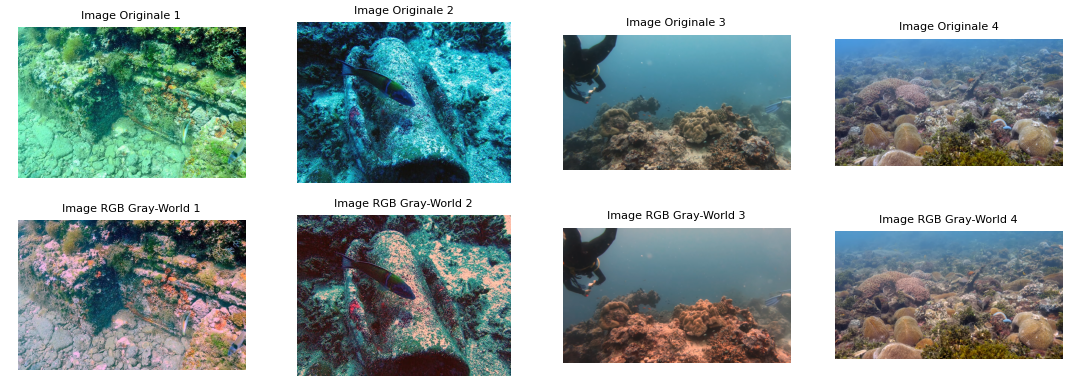
\includegraphics[width=11cm]{image004.png}
\label{figure2.1}
\caption{Résultats de la correction RGB (avec l'hypothèse du monde gris) sur des images sous-marines}
\end{figure} 
\end{center}
\end{frame}


\subsection{Hypothèse des White Patches}
\begin{frame}{Hypothèse des White Patches}
L’hypothèse des White Patches repose sur l’idée que certaines zones de l’image devraient être proches du blanc, même sous un éclairage non uniforme. En ajustant ces zones lumineuses (les "patchs blancs") pour qu'elles correspondent à un blanc idéal, on peut corriger les dominantes de couleur. Sur le principe on identifie les zones les plus lumineuses de l’image et on les ajuste pour qu’elles correspondent à un point blanc idéal \([255, 255, 255]\). Cela permet de corriger les dominantes de couleur sans affecter les autres zones de l’image.
\end{frame}

\begin{frame}{Hypothèse des White Patches}
\begin{enumerate}
    \item \textbf{Conversion en niveaux de gris :} L'image est d'abord convertie en niveaux de gris pour identifier les zones les plus lumineuses.
    
    \item \textbf{Identification des patchs lumineux :} On sélectionne les \( p\% \) des pixels les plus lumineux comme étant les "patchs blancs" :
    \[
P_{\text{bright}} = \left\{ x \in \{1, \dots, N\} \mid \text{Gray}(x) \geq \theta \right\}
\]

    \item \textbf{Calcul de la moyenne des patchs lumineux :} La moyenne des couleurs des patchs lumineux est calculée :
\begingroup
\small   
    $$
    \bar{R}_{\text{bright}} = \frac{1}{\#P_{\text{bright}}} \!\sum_{x\in P_{\text{bright}}}\!\!\!\! R(x) \quad\quad \bar{G}_{\text{bright}} = \frac{1}{\#P_{\text{bright}}}\! \sum_{x\in P_{\text{bright}}} \!\!\!\!G(x) 
    $$
    $$
   \bar{B}_{\text{bright}} = \frac{1}{\#P_{\text{bright}}}\! \sum_{x\in P_{\text{bright}}} \!\!\!\! B(x)
    $$
\endgroup

    \item \textbf{Application de la correction :} Un facteur de correction est appliqué à l'image pour ajuster les canaux \( R \), \( G \), et \( B \) qui est un réajustement du point blanc idéal.
\begingroup
\small   
    $$
    R_{\text{corr}}(x) = R(x) \times \frac{255}{\bar{R}_{\text{bright}}} \quad\quad\quad G_{\text{corr}}(x) = G(x) \times \frac{255}{\bar{G}_{\text{bright}}} \quad\quad\quad B_{\text{corr}}(x) = B(x) \times \frac{255}{\bar{B}_{\text{bright}}}
    $$
\endgroup
\end{enumerate}
\end{frame}

\begin{frame}{Hypothèse des White Patches}
\begin{figure}[h!]
\begin{center}
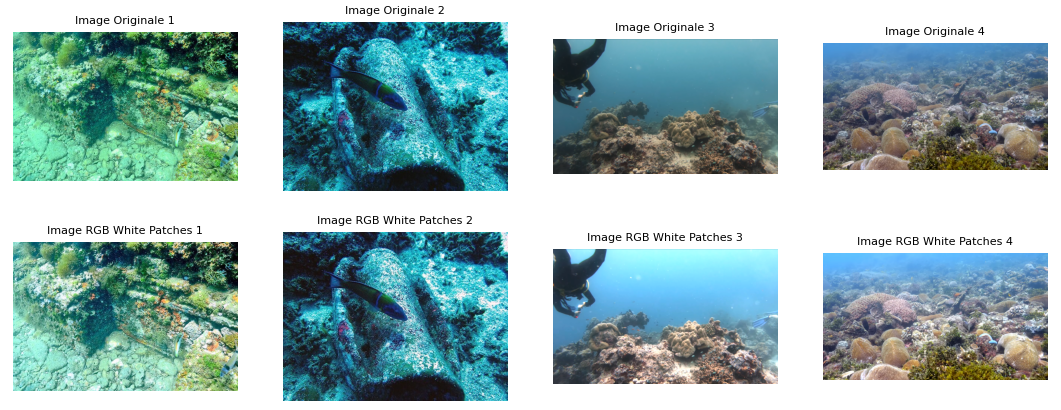
\includegraphics[width=11cm]{image005.png}
\end{center}
\label{figure2.2}
\caption{Résultats de la correction RGB (avec l'hypothèse des white patches $p=2\%$)}
\end{figure}
\end{frame}

\begin{frame}{Hypothèse des White Patches}
\begin{figure}[h!]
\begin{center}
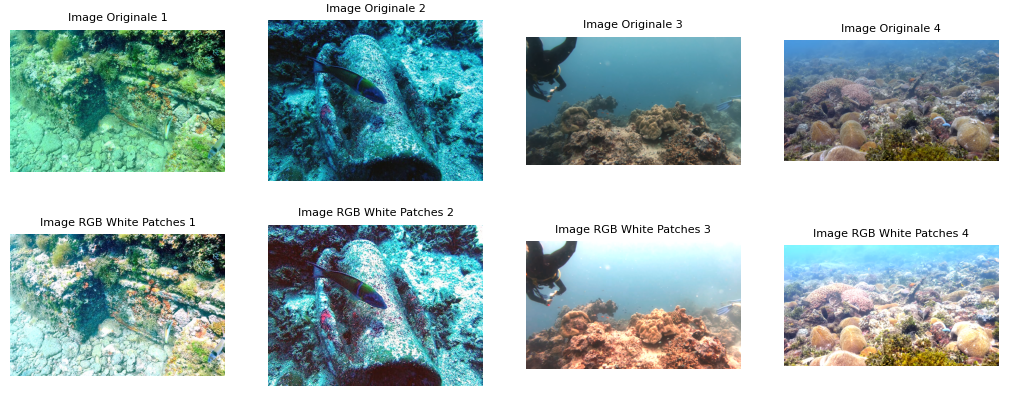
\includegraphics[width=11cm]{image013.png}
\end{center}
\label{figure2.2}
\caption{Résultats de la correction RGB (avec l'hypothèse des white patches $p=20\%$)}
\end{figure}
\end{frame}

\section{Correction des Couleurs à l'Aide de l'Espace \( l\alpha\beta \)}
\frame{\tableofcontents[currentsection]}


\begin{frame}{Correction et Amélioration dans l'Espace \( l\alpha\beta \)}
Cette méthode repose sur une transformation dans l'espace colorimétrique perceptuel $l\alpha\beta$, qui un modèle de couleurs standardisé par la Commission Internationale de l'Éclairage (CIE) en 1976. Contrairement aux espaces colorimétriques comme RGB, qui sont basés sur des caractéristiques physiques de la lumière ou des pigments, l'espace $l\alpha\beta$ cherche à décrire les couleurs de manière plus uniforme et perceptuellement linéaire, ce qui signifie que les différences entre les couleurs dans cet espace correspondent mieux à ce que l'œil humain perçoit.
\end{frame}

\subsection{Conversion dans l'Espace $l\alpha\beta$}
\begin{frame}{Conversion dans l'Espace $l\alpha\beta$}
\par Pour convertir une image RGB en espace \( l\alpha\beta \), plusieurs étapes successives sont effectuées :
\vspace{3mm}
\begin{enumerate}
    \item \textbf{Correction gamma :} Les valeurs RGB sont corrigées pour obtenir des intensités lumineuses linéaires :
    \[
    F'(x) = F(x)^{\frac{1}{\gamma}}
    \]
    \item \textbf{Conversion RGB \(\to\) XYZ :} Les valeurs RGB corrigées sont projetées dans l'espace perceptuel XYZ :
    \[
    X(x) = T_{xyz} \cdot F'(x).
    \]
    \item \textbf{Conversion XYZ \(\to\) LMS :} Une transformation vers l'espace LMS (Long, Medium, Short) des cônes de l'œil humain :
    \[
    L(x) = T_{\text{lms}} \cdot X(x).
    \]
    \item \textbf{Logarithme et PCA :} Les valeurs LMS sont transformées log-linéairement, puis une analyse en composantes principales (PCA) sépare la luminance \( l \) des chromatiques \( \alpha \) (jaune-bleu) et \( \beta \) (rouge-vert) :
    \[
    L_{l\alpha\beta}(x) = T_{\text{pca}} \cdot \log\left(L(x)\right).
    \]
\end{enumerate}
\end{frame}

\subsection{Correction et Amélioration dans l'Espace \( l\alpha\beta \)}
\begin{frame}{Correction et Amélioration dans l'Espace \( l\alpha\beta \)}
Dans l'espace \( l\alpha\beta \), la correction des couleurs se fait en ajustant les canaux \( \alpha \) et \( \beta \), qui représentent respectivement les variations chromatiques jaune-bleu et rouge-vert. Deux méthodes de correction sont appliquées : l'hypothèse du \textbf{monde gris} et l'hypothèse des \textbf{white patches}.

\end{frame}

\begin{frame}{Correction et Amélioration dans l'Espace \( l\alpha\beta \)}
\textbf{Hypothèse du Monde Gris}
\vspace{3mm}
\par L'idée est que la moyenne des valeurs de \( \alpha \) et \( \beta \) dans une scène équilibrée doit être nulle, permettant ainsi de supprimer les dominantes de couleur. La correction se fait en soustrayant la moyenne des valeurs des canaux \( \alpha \) et \( \beta \) :
   \[
   \alpha^*(x) = \alpha(x) - \bar{\alpha} \quad\quad\quad \beta^*(x) = \beta(x) - \bar{\beta}
   \]
\end{frame}

\begin{frame}{Correction et Amélioration dans l'Espace \( l\alpha\beta \)}
\textbf{Hypothèse du Monde Gris}
\vspace{3mm}
\begin{figure}[h!]
\begin{center}
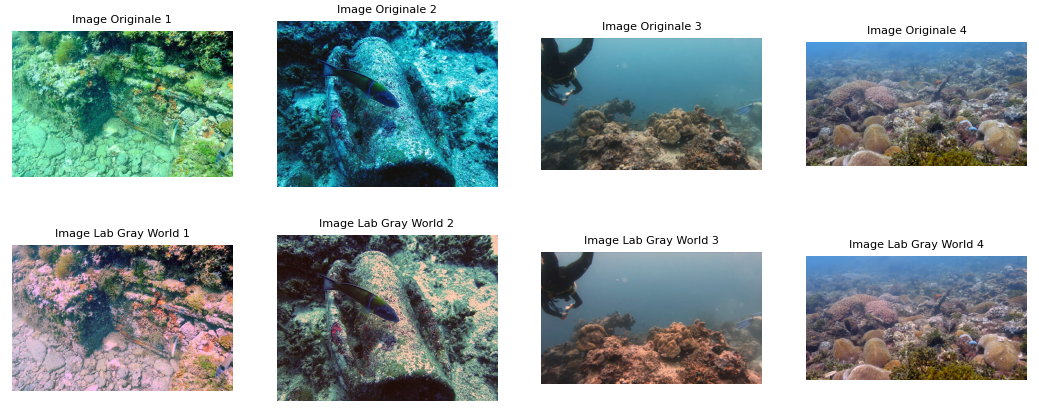
\includegraphics[width=11cm]{image006.png}
\end{center}
\label{figure3.1}
\caption{Résultats de la correction $l\alpha\beta$ (avec l'hypothèse du monde gris) sur des images sous-marines}
\end{figure}
\end{frame}

\begin{frame}{Correction et Amélioration dans l'Espace \( l\alpha\beta \)}
\textbf{Hypothèse du Monde Gris}
\begin{figure}[h!]
\begin{center}
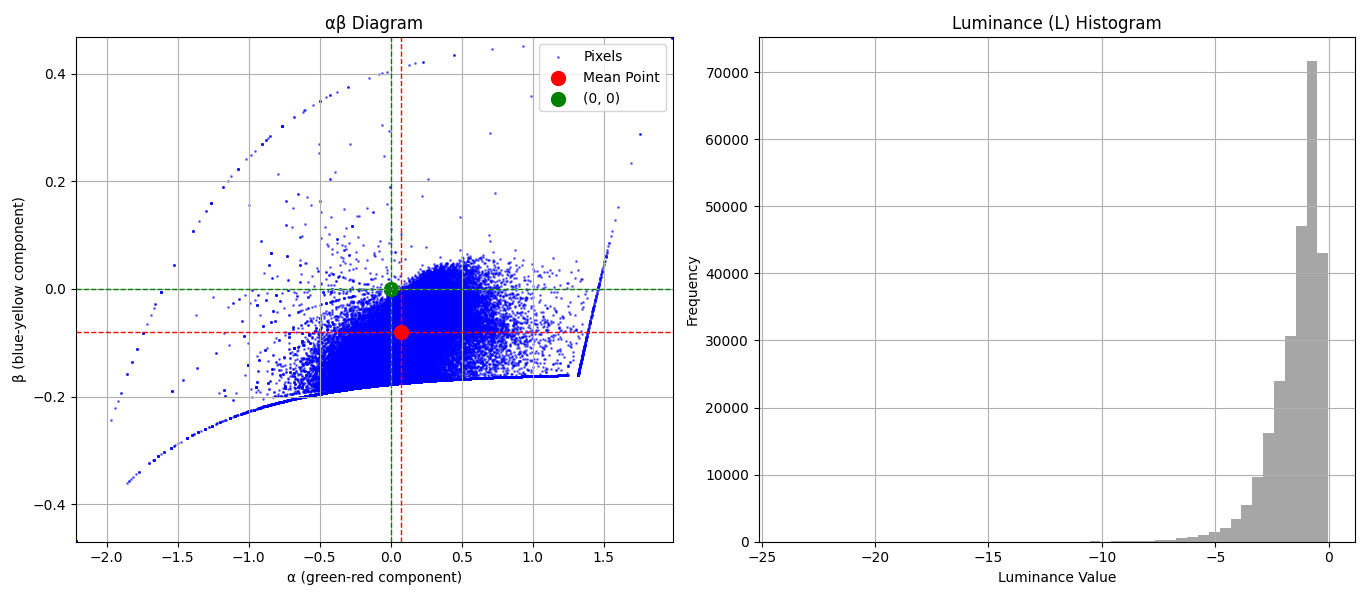
\includegraphics[width=11cm]{image007.png}
\end{center}
\label{figure3.2}
\caption{Diagramme $\alpha\beta$ et Histogramme de la Luminance avant la correction}
\end{figure}
\end{frame}

\begin{frame}{Correction et Amélioration dans l'Espace \( l\alpha\beta \)}
\textbf{Hypothèse du Monde Gris}
\begin{figure}[h!]
\begin{center}
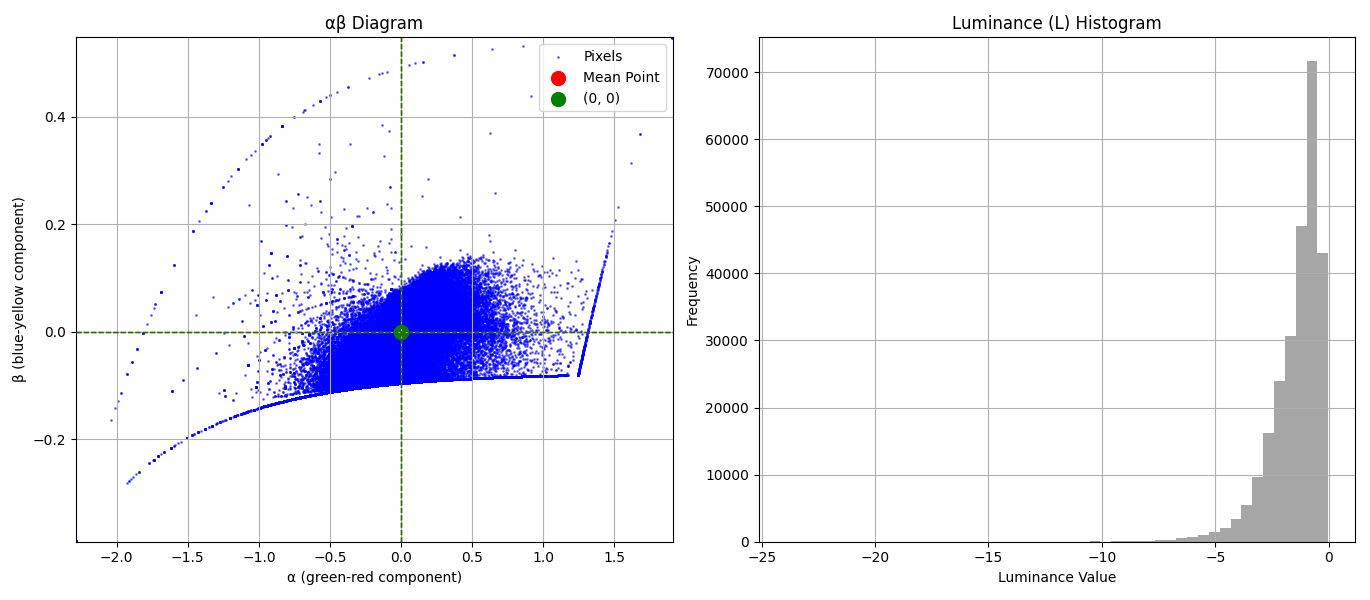
\includegraphics[width=11cm]{image008.png}
\end{center}
\label{figure3.3}
\caption{Diagramme $\alpha\beta$ et Histogramme de la Luminance après la correction}
\end{figure}
\end{frame}

\begin{frame}{Correction et Amélioration dans l'Espace \( l\alpha\beta \)}
\textbf{Hypothèse des White Patches}
\vspace{3mm}
\par Cette méthode ajuste les canaux \( \alpha \) et \( \beta \) en fonction des pixels les plus lumineux (les "patchs blancs"). On identifie les \( p\% \) des pixels les plus lumineux, puis on calcule la moyenne des canaux \( \alpha \) et \( \beta \) pour ces pixels lumineux :
   \[
   \alpha^*(x) = \alpha(x) - \bar{\alpha}_{\text{bright}} \quad\quad\quad \beta^*(x) = \beta(x) - \bar{\beta}_{\text{bright}}
   \]
   où \( \bar{\alpha}_{\text{bright}} \) et \( \bar{\beta}_{\text{bright}} \) sont les moyennes des canaux \( \alpha \) et \( \beta \) pour les pixels lumineux, identifiés en fonction de leur luminance.
\end{frame}

\begin{frame}{Correction et Amélioration dans l'Espace \( l\alpha\beta \)}
\textbf{Hypothèse des White Patches}
\vspace{3mm}  
\begin{figure}[h!]
\begin{center}
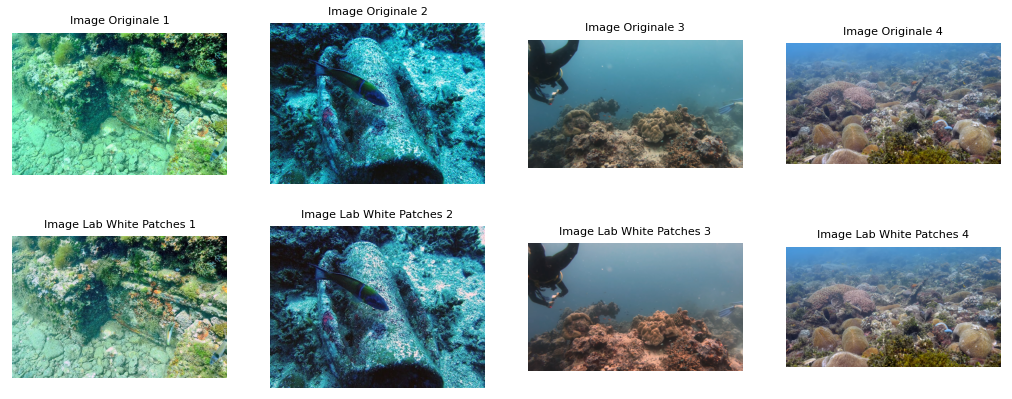
\includegraphics[width=11cm]{image012.png}
\end{center}
\label{figure2.d3}
\caption{Résultats de la correction $l\alpha\beta$ (avec l'hypothèse des white patches avec $p=2\%$) }
\end{figure}
\end{frame}

\begin{frame}{Correction et Amélioration dans l'Espace \( l\alpha\beta \)}
\textbf{Hypothèse des White Patches}
\vspace{3mm}  
\begin{figure}[h!]
\begin{center}
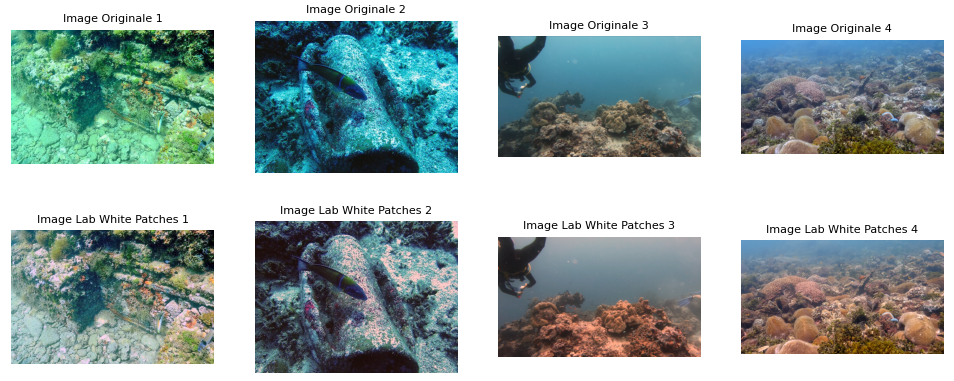
\includegraphics[width=11cm]{image011.png}
\end{center}
\label{figure2.s3}
\caption{Résultats de la correction $l\alpha\beta$ (avec l'hypothèse des white patches avec $p=20\%$) }
\end{figure}
\end{frame}

\begin{frame}{Correction et Amélioration dans l'Espace \( l\alpha\beta \)}
\textbf{Égalisation d'Histogramme sur le Canal \( l \)}
\vspace{3mm}  
\par Pour améliorer le contraste des images corrigées, une égalisation d'histogramme a été appliquée au canal \( l \) des images traitées selon l'hypothèse du monde gris. Cette opération vise à redistribuer les valeurs de luminance de manière à mieux occuper la plage dynamique disponible.
\vspace{2mm}
\par Soit \( l : \Omega \to [0, 1] \), où \( \Omega \) est le domaine de l'image et les intensités du canal $l$ sont normalisées dans l'intervalle \([0, 1]\). L'égalisation d'histogramme est effectuée via le calcul de l'histogramme cumulé \( F \), défini comme :
\[
F(t) = \frac{1}{\# \Omega} \; \# \{x \in \Omega : I(x) \leq t \}, \quad\quad t \in [0, 1],
\]
L'image égalisée est obtenue en appliquant \( F \) sur \( I(x) \), ce qui donne :
\[
I'(x) = F(I(x)).
\]

Lorsque \( F \) est inversible, l'image résultante \( I'(x) \) possède des intensités uniformément réparties, car :
\[
P(F(I) \leq t) = F(F^{-1}(t)) = t.
\]
\end{frame}

\begin{frame}{Correction et Amélioration dans l'Espace \( l\alpha\beta \)}
\begin{figure}[h!]
\begin{center}
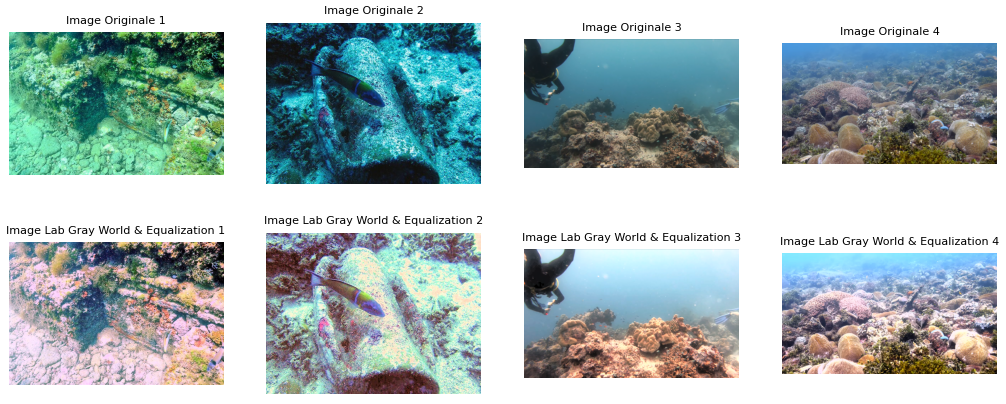
\includegraphics[width=11cm]{image009.png}
\end{center}
\label{figure3.4}
\caption{Résultats de l'égalisation d'histogramme sur le canal $l$ des images $l\alpha\beta\;$ GW}
\end{figure} 
\end{frame}

\section{Méthode ACE : Égalisation Automatique des Couleurs}
\frame{\tableofcontents[currentsection]}
\begin{frame}{Méthode ACE : Égalisation Automatique des Couleurs}
\par Une autre technique qui pourrait nous être utile pour la correction des images sous-marines est l'Automatic Color Equalization (ACE), une méthode conçue pour améliorer à la fois les couleurs globales et locales. Inspirée par les processus visuels humains, ACE combine deux fonctions essentielles : \textbf{la constance des couleurs}, qui assure une perception cohérente des teintes malgré les variations d'éclairage, et \textbf{l'égalisation de la luminosité}, qui ajuste dynamiquement les contrastes de l'image.
\vspace{2mm}
\par ACE fonctionne en calculant une nouvelle valeur pour chaque pixel en tenant compte des contributions des autres pixels, pondérées par leur distance spatiale et leur différence chromatique. En s'appuyant sur des approches traditionnelles de correction globale telles que \textbf{Gray World} et \textbf{White Patch}, ACE élimine efficacement les dominantes de couleur tout en maintenant un contraste équilibré, tant sur le plan global que local.
\end{frame}

\subsection{Modèle et Formulation Mathématique}
\begin{frame}{Modèle et Formulation Mathématique}
\par L'algorithme ACE repose sur une formulation mathématique qui calcule une nouvelle valeur pour chaque pixel d'une image en tenant compte de la distribution spatiale et chromatique de tous les autres pixels. Pour chaque pixel \( x \), la valeur corrigée \( R(x) \) est donnée par :

$$
R(x) = \displaystyle\sum_{y \in \Omega / x}\dfrac{ s_\alpha(I(x) - I(y))}{d(x-y)}, \quad\quad x\in \Omega
$$

\par La pondération spatiale permet de moduler l'influence des pixels voisins en fonction de leur distance et de leur intensité relative. Cette combinaison garantit une correction équilibrée entre les ajustements globaux et locaux.
\vspace{2mm}
\par Après avoir calculé \( R(x) \), les valeurs sont étirées pour occuper la plage dynamique complète de l'image, généralement entre 0 et 1, avec :

$$
L(x) = \frac{R(x) - \min R}{\max R - \min R}
$$
\par L'algorithme ACE, dans sa forme brute, présente une complexité élevée de \( O(N^4) \), ce qui le rend impraticable pour des images de grande taille.
\end{frame}

\begin{frame}{Modèle et Formulation Mathématique}
\begin{figure}[h]
\begin{center}
\begin{tikzpicture}[scale=1]
    % Axes
    \draw[->] (-3, 0) -- (3, 0) node[right] {\(\Delta I\)};
    \draw[->] (0, -2) -- (0, 2) node[above] {\(s_\alpha(\Delta I)\)};
    
    % Lignes grilles
    \draw[gray, dashed] (-3, 1.5) -- (3, 1.5);
    \draw[gray, dashed] (-3, -1.5) -- (3, -1.5);
    \draw[gray, dashed] (-1, -2) -- (-1, 2);
    \draw[gray, dashed] (1, -2) -- (1, 2);
        
    % Labels
    \node[below left] at (-1, 0) {$-\frac{1}{\alpha}$};
    \node[below right] at (1, 0) {$\frac{1}{\alpha}$};
    \node[below] at (-3, 0) {-1};
    \node[below] at (3, 0) {1};
    
    %Fonction
    \draw[red, very thick] (-3, -1.5) -- (-1, -1.5);
    \draw[red, very thick] (3, 1.5) -- (1, 1.5);
    \draw[red, very thick] (-1, -1.5) -- (1, 1.5);


\end{tikzpicture}
\end{center}
\label{figure4.1}
\caption{Fonction pente $s_\alpha$}
\end{figure} 
\end{frame}

\subsection{Fonction Pente Polynomiale}
\begin{frame}{Fonction Pente Polynomiale}
\par Pour résoudre ce problème, la fonction de pente \( s_\alpha \) est approximée par un polynôme, ce qui simplifie les calculs tout en conservant une précision suffisante. Cette approximation réduit la complexité de l'algorithme à \( O(N^2 \log N) \) en utilisant la transformée discrète du cosinus (DCT) pour les convolutions.
\end{frame}

\begin{frame}{Fonction Pente Polynomiale}
\textbf{Gestion des Bords de l'Image}
\vspace{3mm}
\par Lors des convolutions sur une image, la gestion des bords est un défi. L'extension symétrique à demi-échantillon consiste à répliquer les pixels de bord de manière symétrique en miroir à l'extérieur de l'image pour éviter les artefacts causés par une simple périodisation on un padding.
\vspace{2mm}
\par Donc si l'image est de taille $N\times M$ le nouveau domaine \( \mathbb{T}^2 \) qui fait référence à l'ensemble des positions de pixels dans l'image utilisées pour calculer \( R(x) \), est un tore $(2N\!\times\! 2M)$-périodique. 

$$
R(x) = \sum_{y \in \mathbb{T}^2} \omega(x - y)s_\alpha(I(x) - I(y)), \quad x \in \mathbb{T}^2
$$
où $\,\omega : \mathbb{T}^2 \longrightarrow \mathbb{R}_{+}\,$ est une pondération définie par :
$$
\omega(x - y) =
\begin{cases}
0 & \text{si } x = y \\
\dfrac{1}{d(x - y)} & \text{si } x \neq y
\end{cases}
$$
\end{frame}

\begin{frame}{Fonction Pente Polynomiale}
\textbf{Approximation Polynomiale}
\vspace{3mm}
\par La fonction de pente $s_\alpha$ est approximée par un polynôme impair, ce qui simplifie les calculs tout en maintenant une précision suffisante. Cette approximation minimise l'erreur maximale sur l'intervalle \([-1, 1]\) en optimisant les coefficients \( c_m \) du polynôme.
$$
\min_{c} \max_{t \in [-1, 1]} \left| s_\alpha(t) - \sum_{m=1}^{D} c_m t^m \right|
$$
Les coefficients optimaux du polynôme pour différentes valeurs de \( \alpha \) peuvent être obtenus via des méthodes d'optimisation telles que l'algorithme de Remez.
\end{frame}

\begin{frame}{Fonction Pente Polynomiale}
\textbf{Calcul avec les Convolutions}
\vspace{3mm}
\par Cette approximation polynomiale permet de décomposer \( R(x) \) en une somme de convolutions :

$$
R(x) = \sum_{n=0}^{D} a_n\left(I(x)\right) \left( \omega * I^n \right)(x)
$$

où :
\begin{itemize}
\item[$\bullet$] \( \omega * I^n \) est une convolution cyclique sur \( \mathbb{T}^2 \).
\item[$\bullet$]  \( a_n\left(t\right) \) un polynôme défini par :
$$
\sum_{m=n}^{D} c_m \binom{m}{n} (-1)^{m-n+1} t^{m-n}
$$
\end{itemize}

 Les convolutions peuvent être efficacement calculées avec les transformations DCT en \( O(N^2 \log N) \) opérations.et pour une image couleur RGB, \( 3M \) convolutions doivent être calculées. La sommation sur \( n \) peut être parallélisée, puisque l'évaluation de \( a_n(x) \left( \omega * I_n \right)(x) \) est indépendante pour chaque \( n \).
\end{frame}


\subsection{Implémentation pour la Correction des Images Sous-marines}
\begin{frame}{Implémentation pour la Correction des Images Sous-marines}
\textbf{Test de l'ACE sur des Images Synthétiques}
\vspace{3mm}
\par La méthode ACE a été initialement implémentée pour des images synthétiques afin d'évaluer son efficacité dans des conditions idéales et d'observer les caractéristiques du filtrage. Certaines de ces propriétés dépendent des paramètres de l'algorithme, tandis que d'autres sont influencées par le contenu de l'image. À moins d'indication contraire, les résultats présentés dans ici utilisent :
\vspace{3mm}
\begin{itemize}
	\item[$\bullet$] $\,\alpha = 7$.
    \item[$\bullet$]  Un polynôme $c$ de degré $D = 11$. 
    \item[$\bullet$]  Une distance euclidienne.
\end{itemize}
\end{frame}

\begin{frame}{Implémentation pour la Correction des Images Sous-marines}
\begin{figure}[h]
\begin{center}
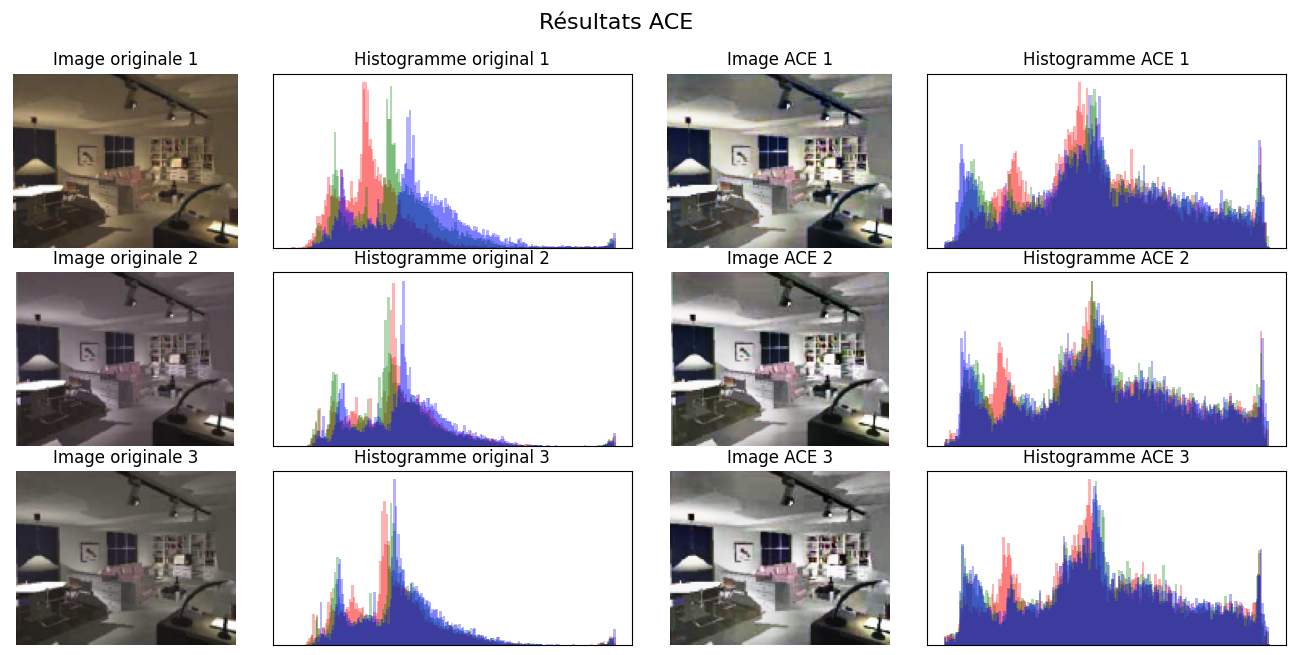
\includegraphics[width=11cm]{image001.png}
\end{center}
\label{figure4.2}
\caption{Résultats de l'ACE sur des images synthétiques}
\end{figure}
\end{frame}

\begin{frame}{Implémentation pour la Correction des Images Sous-marines}
\textbf{Correction des Images Sous-marines avec l'ACE}
\vspace{3mm}
\begin{figure}[h!]
\begin{center}
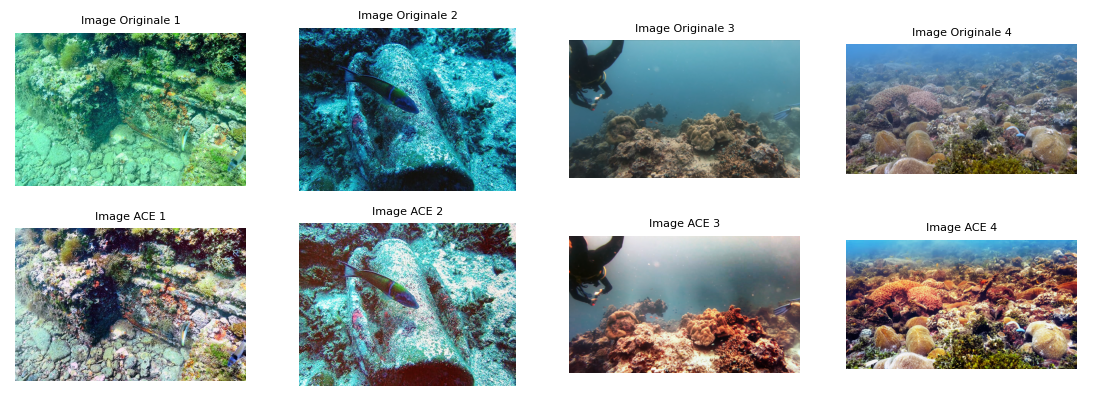
\includegraphics[width=11cm]{image002.png}
\end{center}
\label{figure4.3}
\caption{Résultats de l'ACE sur les images sous-marines}
\end{figure} 
\end{frame}


\begin{frame}{Implémentation pour la Correction des Images Sous-marines}
\textbf{Application de l'ACE sur le Canal \( l \)}
\vspace{3mm}
\par Une autre approche implémentée consiste à appliquer l'ACE uniquement sur le canal $\,l\,$ après une transformation dans l'espace colorimétrique $l\alpha\beta$, dans le but d'améliorer le contraste et la luminosité de l'image, tout en supposant l'hypothèse du monde gris.
\end{frame}

\begin{frame}{Implémentation pour la Correction des Images Sous-marines}
\begin{figure}[h!]
\begin{center}
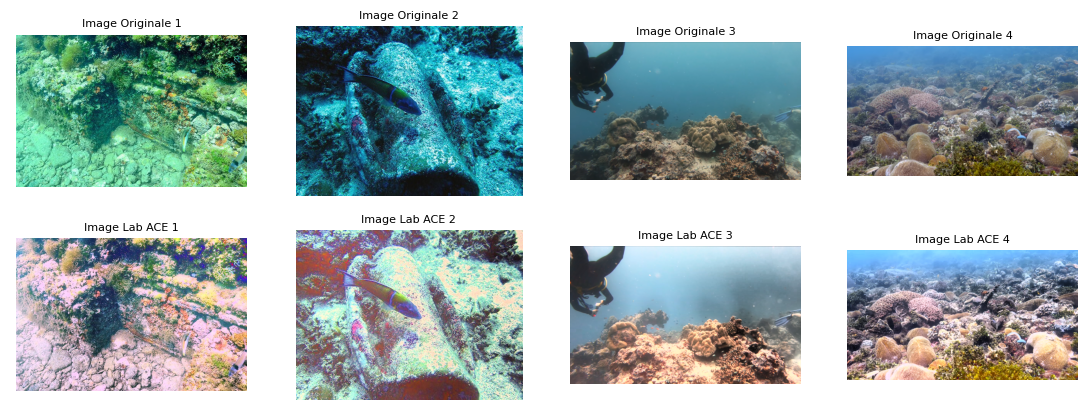
\includegraphics[width=11cm]{image003.png}
\end{center}
\label{figure4.4}
\caption{Résultats de l'ACE sur le canal $l$ des images $\l\alpha\beta\;$GW}
\end{figure} 
\end{frame}

\section{Conclusion}
\begin{frame}{Conclusion}
\par Lorsque l’on s’oriente vers des applications en temps réel, comme l’analyse de vidéos pour des robots sous-marins ou des systèmes de surveillance, la rapidité des algorithmes devient un critère essentiel. Les méthodes classiques, bien qu'efficaces dans des contextes spécifiques, peinent à répondre à cette exigence en raison du temps de traitement nécessaire. De ce fait, une approche moderne, basée sur l’exploitation de modèles d’apprentissage profond préalablement entraînés, s’impose comme une solution prometteuse. Ces modèles permettent de combiner \textbf{efficacité}, \textbf{rapidité} et \textbf{qualité}.
\end{frame}

\end{document}
